\documentclass[12pt]{article}
\usepackage[T1]{fontenc}
%\usepackage[latin9]{inputenc}
\usepackage[utf8]{inputenc}
\usepackage[english]{babel}
\usepackage{amsmath}
%\usepackage{halloweenmath}
\usepackage{amsfonts}
\usepackage{amssymb}
%\usepackage{setspace}
\usepackage{rotating}
\usepackage{graphics}
\usepackage{eurosym}
\usepackage[round]{natbib}
%\usepackage{graphicx}
%\usepackage{float} 				%allows you to float images
\usepackage{latexsym}
%\usepackage{bbding}
%\usepackage {moresize}
\usepackage{listings}
\usepackage{bbding}
\usepackage{blindtext}
\usepackage{hhline}
\usepackage{tikz}
\usetikzlibrary{trees}
%\usetikzlibrary{shapes,backgrounds}
%\usepackage{pgfplots}
%\usetikzlibrary{arrows}
\usepackage{enumitem}
%\doublespacing
%\usepackage{geometry}
\usepackage{amsthm}
\usepackage{color}
%\usepackage{array,multirow}
\usepackage{subcaption}
%\usepackage{pst-plot}
%	\psset{xunit=15mm}
%\geometry{verbose,tmargin=1in,bmargin=1in,lmargin=.5in,rmargin=.5in}
\setlength{\parskip}{\bigskipamount}
\setlength{\parindent}{0pt}
\usepackage{multicol}


\newenvironment{problem}[3][Problem]{\begin{trivlist}
\item[\hskip \labelsep {\bfseries #1}\hskip \labelsep {\bfseries #2.}]}{\end{trivlist}}

\newcommand{\barr}{\bar{r}}
\newcommand{\ddx}{\frac{d}{dx}}
\newcommand{\infsum}{\sum_{n=1}^{\infty }}

\title{Problem Set 10 \thanks{Problems:13.1, 13.5, 13.6, 13.11, 13.25}}
\author{Ian McGroarty \\
	Course Number: 555.444 \\
}
\date{November 4, 2019}

\begin{document}

\maketitle
%%%%%%%%%%%%%%%%%%%%%%%%%%%%%%%%%%%%%%%%%%%%%%%%%%%%%%%%
%%%%%%%%%%%%%%%%%%%%%%%%%%%%%%%%%%%%%%%%%%%%%%%%%%%%%%%%
%%%%%%%%%%%%%%%%%%%%%%%%%%%%%%%%%%%%%%%%%%%%%%%%%%%%%%%%

\newpage
\begin{problem}{14.3}. $a = 0.5, b = 4.0$ How high does the company\rq{}s initial cah postion have to be for th company to have less than a 5\% change of a negative cahs potion by the end of one year ($\Delta t = 4$) . The math here is pretty simple, the concept too a minute for me to wrap my head around. See figure 1, the purple line is the expected value of the stock over the 4 quarters (1 year). I drew a normal distribution with mean at ($S_0+2$) and a variance of 16 to illustrate the probability distribution at quarter 4. This turns the problem into a simple normal distribution problem. 
\begin{align*}
\frac{\Delta S}{S} & ~\sim \Phi (\mu \Delta t , \sigma^2 \Delta t) && \text{Eqn. 14.9 pg} \\
\frac{\Delta S}{S} & ~\sim \Phi (0.5 \cdot 4 , 4\cdot 4) \\
\frac{\Delta S}{S} & ~\sim \Phi (2, 16) \\
P(a \leq Y) &= P(\frac{a-\mu }{\sigma} \leq \frac{Y- \mu }{\sigma } && \text{Larsen, Mark (2018) Def. 4.3.1 pg 249} \\
P(\frac{Y- \mu }{\sigma } &\leq \hat  -1.64) = 0.05 &&\text{using qnorm(0.05,0,1) in R} \\
\frac{Y+2}{4} &\leq -1.64 \\
Y &\leq 4.58 \ (million)
\end{align*}
\begin{figure}
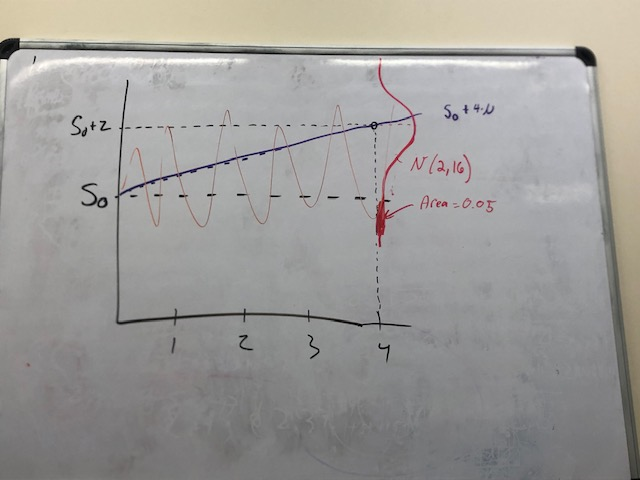
\includegraphics[width=\linewidth]{mod10_p13.png}
\caption{Problem 14.3}
\end{figure}
\end{problem}

\begin{problem}{14.5}. Consider a variable S that follows the process: $$dS = \mu dt + \sigma dz$$
For the first three years, $\mu = 2, \sigma = 3$ for the next 3 years, $\mu = 3, \sigma = 4$. $S_0=5$. What is the probability distribution of the value of the variable at the end of year 6. 

Again, I include a graph to illustrate the logic of this problem. But the math is simple. Since the time is independent, variances and means are additive. 
\begin{align*}
\frac{\Delta S}{S} & ~\sim \Phi (\mu \Delta t , \sigma^2 \Delta t) && \text{Eqn. 14.9 pg} \\
 & \sim \Phi (2 \cdot 3 , 9 \cdot 3) && \text{First 3 years} \\
 & \sim \Phi (6 , 27) \\
 & \sim \Phi (3 \cdot 3 , 16 \cdot 3) && \text{Second 3 years} \\
 & \sim \Phi (9 , 48) \\
& \sim \Phi (9+6 , 48+27)  && \text{components are additive} \\
 & \sim \Phi (15 , 75) \\
\frac{\Delta S}{S}  & \sim \Phi (20 , 75) && \text{add the initial value to the mean}
\end{align*}
\begin{figure}
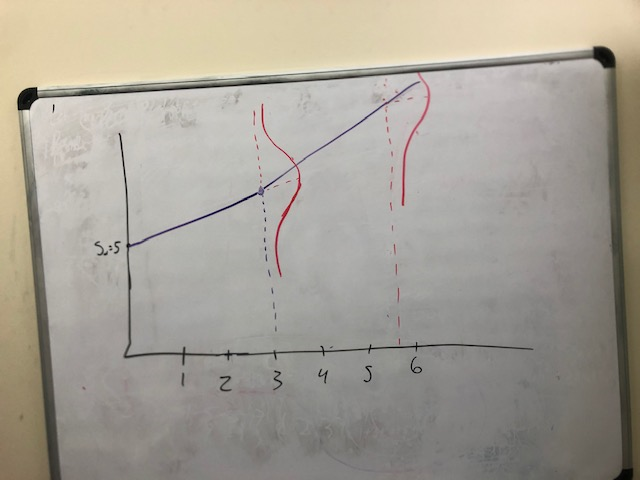
\includegraphics[width=\linewidth]{mod10_p5.png}
\caption{problem 14.5}
\end{figure}
\end{problem}


\begin{problem}{14.9}. It has been suggested that the short-term interest rate,r , follows the stochastic process
$$ dr = a(b-r)dt + rc dz $$
where a , b , and c are positive constants and dz is a Wiener process. Describe the nature
of this process. \\
I\rq{}m not fully sure what you mean by \lq\lq{}describe the nature of the process\rq\rq{} but lets just talk about it. 
the short term interest rate follows a Wiener process with drift $a(b-r)$ and variance $rc$. Focusing a bit on the drift because that is a little interesting. $a(b-r)$ with $a,b,r>0$ suggest that the drift can be negative, $(b<r)$ or positive $(b>r)$ or even zero. If b is constant then that isnt all that interesting, but if you think about b as a function of time or something that could make things more complicated but more dynamic as well!
\end{problem}

\newpage 
\begin{problem}{14.11}. Suppose that x is the yield to maturity with continuous compounding on a zero-coupon bond
that pays off \$1 at time T . Assume that x follows the process: $$ dx = a(x_0 - x)dt + sxdz$$ 
Alright so lets take this as an opportunity to talk through this a bit. A bond with a yield to maturity x is priced as $B=e^{-x(T-t)}$. x follows a Wiener process with drift $a(x_0 - x)$ and variance $sx$. By Ito\rq{}s lemma we can find the process for the Bond price with this yield to maturity. First we will define the derivatives we will need and then walk through the Ito process:
\begin{align*}
B &= e^{-x(T-t)} \\
\frac{\partial B}{\partial x} &= -(T-t)e^{-x(T-t)}  = -(T-t)\cdot B \\
\frac{\partial^2 B}{\partial x^2} &= (T-t)^2e^{-x(T-t)} = (T-t)^2\cdot B \\
\frac{\partial B}{\partial t} &= x e^{-x(T-t)} = xB \\
dB &= (\frac{\partial B}{\partial x} [a(x_0-x)] + \frac{\partial B}{\partial t} + \frac{1}{2} \frac{\partial^2 B}{\partial x^2}[(sx)^2])dt + \frac{\partial B}{\partial t}[sx]dt \\t
dB &= ((-(T-t)\cdot B) [a(x_0-x)] + xB+ \frac{1}{2} ( (T-t)^2\cdot B)[(sx)^2])dt +(xB)[sx]dt 
\end{align*}
\end{problem}

\begin{problem}{14.13}. Expected return is \%16, volatility is \%30, $S_t = \$50$. 
\begin{align*}
\textbf{(a)} & E(S_{t+1} = S_t + S_t\cdot \mu = 50 + 50\cdot (0.16/365) = \$ 50.022 \\
\textbf{(b)} & \sigma_{t+1} = S_t \sigma^2 \cdot \sqrt(t) = 50\cdot 0.3 \cdot \sqrt (1/365) = 0.785 \\
\textbf{(c)} & \mu \pm z_{0.95}\cdot \sigma = 50.022 \pm 1.96\cdot 0.785 = (48.483,51.561)
\end{align*}
\end{problem}
\end{document}